\scanpage{44}
% archive foliation: 43
\figure{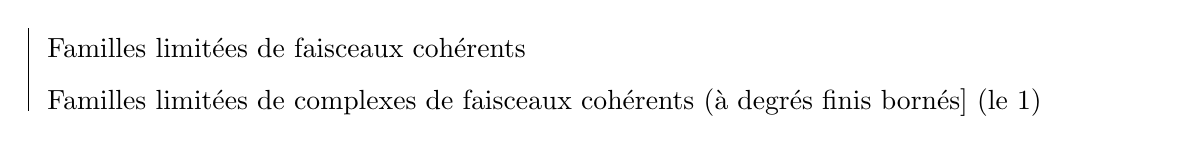
\begin{tikzpicture}
\draw (0,0.25)--(0,-0.8);
\node[anchor=west] at (0.12,0) {Familles limitées de faisceaux cohérents};
\node[anchor=north west,text width=14cm] at (0.12,-0.4) {Familles limitées de complexes de faisceaux cohérents \inserted{(\unsure{à} degrés \deleted{finis} bornés]} (\unsure{le} \illegible{1})};
\end{tikzpicture}}

\uline{Prop. 1} Réunion finie de familles limitées est limitée.

\uline{Prop 2} Possibilité dans la définition de supposer \deleted{\unsure{$S$ réduit}} des \deleted{familles} ``familles \unsure{virtuelles}'' plates sur $T$

\uline{Prop. 3} Changement de base \inserted{$S'\longrightarrow S$} transforme famille limitée en famille limitée. Réciproque si $\operatorname{Im}(S'-S)$ contient tous les points de $S$ intervenant dans $F$

\uline{Prop 4} $H^p(K)$

\uline{Prop. 5} $H^{S\,p}_{f_1,-,f_n}(K_1,-,K_n)$, si $f_i:X_i\unsure{-|\longrightarrow}X$ est propre, $K_i$ sur $X_i$.

\uline{Cor. 1} \deleted{\unsure{$L$}} Tors locaux \deleted{\unsure{$n$}}

\uline{Cor 2} Images inverses par $X'-X$

\uline{Cor 3} Images directes et $\underline{\underline R}^p f_*$

\figure{\begin{tikzpicture}\draw (0.3,0.6)--(0,0.35)--(0.8,-0.9);\end{tikzpicture}}

\uline{Prop 6} $\underline{\operatorname{Ext}}^p_{\underline O_X}(K,L)$ \hfill $[$

\uline{Cor.} $\underline{\operatorname{Hom}}(F,G)$

\uline{Prop 7} $\underline{\operatorname{Ext}}^p_{\unsure{O_X|e_X},f}(K,L)$ quand ça marche

Cor. $\underline{\operatorname{Ext}}^1_{\unsure{O_X|e_X},f}(F,G)$ en tous cas.
